%% =====================================================================
%%  Báo cáo khoa học — Đề tài hoạt động nhóm
%%  Mẫu: ACM Conference Proceedings (sample-sigconf, acmart)
%%  Đề tài: Dự báo Giá Bất động sản Việt Nam và Hoa Kỳ bằng
%%          Học máy Tích hợp (Stacking & Boosting Ensembles)
%%
%%  Engine khuyến nghị: xelatex (để hỗ trợ tiếng Việt qua Libertine).
%%  Build:  make            (sử dụng latexmk)
%%          make clean
%% =====================================================================
\documentclass[sigconf,nonacm]{acmart}

%% ----- Vietnamese / Unicode support (xelatex) ------------------------
%% acmart đã nạp sẵn fontspec + Libertine, vốn hỗ trợ đầy đủ ký tự
%% Tiếng Việt. Chúng ta chỉ cần khai báo ngôn ngữ qua polyglossia.
\usepackage{polyglossia}
\setdefaultlanguage{vietnamese}
\setotherlanguage{english}

%% ----- Các gói bổ sung -----------------------------------------------
\usepackage{booktabs}
\usepackage{multirow}
\usepackage{graphicx}
\usepackage{subcaption}
\usepackage{amsmath}
\usepackage[ruled,linesnumbered]{algorithm2e}

%% ----- BibTeX: tránh lỗi với polyglossia ----------------------------
\AtBeginDocument{\providecommand\BibTeX{{Bib\TeX}}}

%% ----- Thông tin xuất bản (placeholder; điều chỉnh khi nộp) ----------
\setcopyright{none}
\copyrightyear{2025}
\acmYear{2025}
\acmConference[CTK46B-PM 2025]%
              {Học phần Phương pháp Học máy --- Đề tài cuối kỳ}%
              {Tháng 10, 2025}{Việt Nam}
\acmISBN{}
\acmDOI{}

%% ----- Bài báo bắt đầu -----------------------------------------------
\begin{document}

\title{Dự báo Giá Bất động sản Việt Nam và Hoa Kỳ\\
       bằng Học máy Tích hợp:\\
       Nghiên cứu so sánh giữa Stacking và Boosting Ensembles}

\subtitle{Forecasting Housing Prices in Vietnam and the United States via
          Ensemble Learning: A Comparative Study of Stacking and Boosting}

%% --- Tác giả: lấy từ README.md, để trống dòng affiliation cho nhóm --
\author{Đồng Gur Hà Hải}
\affiliation{%
  \institution{Lớp CTK46B-PM --- Học phần Phương pháp Học máy}
  \city{}
  \country{Việt Nam}
}
\email{hai.dgh.2212363@example.edu.vn}

%% Nếu là nhóm có thêm thành viên, bổ sung khối \author{} kế tiếp
%% theo mẫu sau (xóa dấu \iffalse \fi để bật):
\iffalse
\author{Tên Thành Viên 2}
\affiliation{\institution{Lớp CTK46B-PM}\country{Việt Nam}}
\email{thanhvien2@example.edu.vn}
\fi

%% ============ Tóm tắt ============
\begin{abstract}
Bất động sản là một trong những thị trường tài chính phức tạp nhất, với
giá trị tài sản chịu ảnh hưởng phi tuyến của hàng chục yếu tố vĩ mô,
địa lý và pháp lý. Báo cáo này trình bày một nghiên cứu so sánh có hệ
thống giữa các phương pháp \textbf{Học máy tích hợp} (Ensemble Learning)
trên hai thị trường có đặc tính trái ngược: thị trường \emph{Việt Nam}
với dữ liệu cào tự động từ \texttt{batdongsan.com.vn} (1\,000 tin đăng,
nhiều nhiễu, ít đặc trưng cấu trúc) và thị trường \emph{Hoa Kỳ} với bộ
\emph{Ames Housing} chuẩn hóa của cuộc thi Kaggle House Prices
(2\,919 mẫu, 79 đặc trưng). Chúng tôi triển khai bốn thuật toán Boosting
hiện đại (GBM, XGBoost, LightGBM, CatBoost) cùng các kiến trúc tổng hợp
(Voting, Stacking và Blended Stacking) trong cùng một quy trình thử
nghiệm. Kết quả thực nghiệm cho thấy: (i) trên dữ liệu Hoa Kỳ, mô hình
Blended Stacking đạt $R^2 = 0{.}927$ và RMSE\,$=0{.}111$ trên thang
$\log(1+\text{SalePrice})$, vượt xa mọi mô hình đơn lẻ
($R^2 \le 0{.}924$); (ii) việc bổ sung Feature Engineering bậc cao và
chuẩn hóa Box--Cox giúp cải thiện RMSE thêm $\sim 16\%$ so với pipeline
Boosting cơ bản; (iii) trên dữ liệu Việt Nam thô và thiếu đặc trưng,
mô hình Stacking chỉ đạt $R^2 \approx 0{.}087$, cho thấy giới hạn của
học máy khi đặc trưng đầu vào không đủ giàu --- một bài học quan trọng
về tầm quan trọng của giai đoạn thu thập dữ liệu. Báo cáo cũng phân
tích chi phí huấn luyện, mức độ quan trọng của đặc trưng và đề xuất
hướng phát triển dựa trên trích xuất văn bản nâng cao (NLP) cho thị
trường nội địa.
\end{abstract}

%% ============ CCS / Keywords ============
\begin{CCSXML}
<ccs2012>
   <concept>
       <concept_id>10010147.10010257.10010258.10010259.10010264</concept_id>
       <concept_desc>Computing methodologies~Ensemble methods</concept_desc>
       <concept_significance>500</concept_significance>
   </concept>
   <concept>
       <concept_id>10010147.10010257.10010293.10010294</concept_id>
       <concept_desc>Computing methodologies~Boosting</concept_desc>
       <concept_significance>500</concept_significance>
   </concept>
   <concept>
       <concept_id>10010147.10010257.10010293.10010299</concept_id>
       <concept_desc>Computing methodologies~Supervised learning by regression</concept_desc>
       <concept_significance>500</concept_significance>
   </concept>
   <concept>
       <concept_id>10002951.10003317.10003338</concept_id>
       <concept_desc>Information systems~Web mining</concept_desc>
       <concept_significance>300</concept_significance>
   </concept>
</ccs2012>
\end{CCSXML}

\ccsdesc[500]{Computing methodologies~Ensemble methods}
\ccsdesc[500]{Computing methodologies~Boosting}
\ccsdesc[500]{Computing methodologies~Supervised learning by regression}
\ccsdesc[300]{Information systems~Web mining}

\keywords{Bất động sản; Học máy tích hợp; Stacking; Boosting;
  XGBoost; LightGBM; CatBoost; Web Scraping; Feature Engineering;
  Ames Housing; Batdongsan.com.vn}

\maketitle

%% ============ 1. Giới thiệu ============
\section{Giới thiệu}

Định giá bất động sản (BĐS) là một bài toán cốt lõi trong kinh tế đô
thị, ảnh hưởng trực tiếp đến quyết định đầu tư, vay thế chấp, đánh
thuế tài sản và quy hoạch hạ tầng. Khác với cổ phiếu hay tiền tệ, mỗi
căn nhà là một tài sản \emph{không đồng nhất}: giá trị phụ thuộc đồng
thời vào diện tích sàn, chất lượng xây dựng, tuổi nhà, vị trí địa lý
và rất nhiều yếu tố ngầm khó định lượng (thẩm mỹ kiến trúc, môi trường
xung quanh, kỳ vọng về quy hoạch tương lai). Đặc điểm này khiến các
mô hình hồi quy tuyến tính cổ điển thường không đủ năng lực biểu diễn,
trong khi các mô hình \emph{Học máy tích hợp} (Ensemble Learning) đã
trở thành tiêu chuẩn de~facto cho dữ liệu dạng bảng có nhiều đặc trưng
phi tuyến \cite{caruana2006empirical,olson2018data,fernandez2014large}.

\paragraph{Động lực nghiên cứu.}
Hai bộ dữ liệu nổi bật trong cộng đồng minh hoạ rõ hai cực của bài
toán định giá BĐS: \emph{Ames Housing}~\cite{decock2011ames} ---
được sử dụng trong cuộc thi Kaggle House Prices --- là một bộ dữ
liệu \emph{sạch}, có 79 biến giải thích, được dùng làm chuẩn so sánh
cho các thuật toán hồi quy tiên tiến. Ngược lại, các tin đăng trên
\texttt{batdongsan.com.vn} đại diện cho dữ liệu \emph{thực tế tại Việt
Nam}: ngôn ngữ tự nhiên, đơn vị giá lẫn lộn (``10,5 tỷ'', ``500
triệu'', ``Thoả thuận''), và thiếu các trường có cấu trúc về tuổi
nhà, chất lượng xây dựng hay loại sổ đỏ. Việc xây dựng cùng một quy
trình học máy trên hai bộ dữ liệu đối lập như vậy giúp chúng tôi đánh
giá khách quan \emph{ranh giới khả năng và giới hạn} của các phương
pháp tích hợp khi triển khai trong môi trường vận hành thực.

\paragraph{Đóng góp.}
Báo cáo này có ba đóng góp chính:
\begin{enumerate}
  \item Một quy trình \emph{end-to-end} từ Web Scraping đến học máy
    cho thị trường BĐS Việt Nam, với cơ chế phân tích văn bản dựa
    trên biểu thức chính quy (regex) để trích xuất quận/huyện và
    chuẩn hoá đơn vị giá về \emph{triệu VND}.
  \item Một nghiên cứu so sánh có kiểm soát giữa bốn thuật toán
    Boosting (GBM, XGBoost, LightGBM, CatBoost) và ba phương pháp
    tích hợp (Voting, Stacking, Blended Stacking) trên hai bộ dữ
    liệu, sử dụng cùng một giao thức đánh giá (RMSE trên thang $\log
    (1+\text{giá})$).
  \item Phân tích định lượng vai trò của Feature Engineering bậc cao
    và chuẩn hoá Box--Cox đối với mô hình Stacking; đo lường chính
    xác mức cải thiện RMSE và $R^2$ so với baseline Boosting.
\end{enumerate}

\paragraph{Cấu trúc bài báo.}
Phần~\ref{sec:related} điểm qua các công trình liên quan. Phần~\ref{sec:datasets}
mô tả hai bộ dữ liệu. Phần~\ref{sec:method} trình bày quy trình tiền xử
lý và kiến trúc các mô hình. Phần~\ref{sec:experiments} báo cáo kết quả
thực nghiệm và phân tích so sánh. Phần~\ref{sec:discussion} thảo luận
các bài học rút ra. Phần~\ref{sec:conclusion} kết luận và đề xuất
hướng nghiên cứu tiếp theo.

%% ============ 2. Công trình liên quan ============
\section{Công trình liên quan}\label{sec:related}

\paragraph{Boosting cây quyết định.}
Họ thuật toán Boosting --- bắt đầu từ AdaBoost~\cite{freund1997decision}
và Gradient Boosting Machine (GBM) của Friedman~\cite{friedman2001greedy}
--- đã trải qua nhiều cải tiến quan trọng. \emph{XGBoost}
\cite{chen2016xgboost} bổ sung điều tiết $\ell_1, \ell_2$ và song song
hoá việc xây dựng cây. \emph{LightGBM}~\cite{ke2017lightgbm} thay thế
chiến lược phân nhánh cân bằng bằng \emph{leaf-wise} kết hợp histogram
và Gradient-based One-Side Sampling (GOSS), cho phép huấn luyện nhanh
trên các bộ dữ liệu lớn. \emph{CatBoost}~\cite{prokhorenkova2018catboost}
giới thiệu \emph{ordered boosting} và \emph{ordered target statistics} để
xử lý biến phân loại mà không bị rò rỉ thông tin từ tập huấn luyện. Cả
ba thư viện này đã chiếm vị trí thống trị trên các bảng xếp hạng Kaggle
cho dữ liệu dạng bảng~\cite{olson2018data}.

\paragraph{Stacking và Blending.}
\emph{Stacked generalization}~\cite{wolpert1992stacked} là phương pháp
học một mô hình \emph{meta} (tầng 2) trên đầu ra của các mô hình
\emph{cơ sở} (tầng 1) đã được đánh giá thông qua dự báo
out-of-fold. So với Voting/Averaging, Stacking khai thác được tương
quan giữa các mô hình; so với Bagging và Boosting, Stacking cho phép
kết hợp các mô hình \emph{khác họ} (ví dụ Lasso, Ridge, SVR cùng với
GBM)~\cite{breiman1996stacked}. \emph{Blending} là biến thể đơn giản
hóa, sử dụng tập validation cố định thay vì K-fold; tuy ít ổn định hơn
nhưng giảm chi phí huấn luyện và thường được sử dụng để tổng hợp các
giải pháp Stacking sẵn có~\cite{tang2017insurance}.

\paragraph{Học máy cho định giá BĐS.}
Park và Bae~\cite{park2015using} sử dụng C4.5, RIPPER và Naïve Bayes
trên dữ liệu Fairfax County. Nghiên cứu của Truong et al.~\cite{truong2020housing}
trên thị trường Bắc Kinh so sánh Random Forest, XGBoost và một mạng
nơ-ron stacked, cho thấy XGBoost và Stacking vượt trội trong điều
kiện dữ liệu giàu đặc trưng. Tại Việt Nam, các nghiên cứu thực
nghiệm còn khá hạn chế và đa số tập trung vào hồi quy tuyến tính và
Random Forest trên dữ liệu nhỏ; chúng tôi không tìm thấy nghiên cứu
công bố nào áp dụng Stacking với CatBoost cho dữ liệu cào tự động từ
\texttt{batdongsan.com.vn}.

\paragraph{Web scraping cho dữ liệu BĐS.}
Việc cào dữ liệu từ các nền tảng tin đăng đặt ra hai thách thức:
(i) các cơ chế chống bot như Cloudflare và Akamai, và (ii) chuẩn
hoá giá trị từ ngôn ngữ tự nhiên. Các giải pháp như
\texttt{undetected\_chromedriver}~\cite{undetectedcdp} kết hợp giả
lập hành vi người dùng với điều khiển phiên Selenium thực đã được
chứng minh là hiệu quả trong việc thu thập tin đăng quy mô vừa
(${\sim}10^3$ trang) mà không bị chặn~\cite{wahyudi2021scraping}.

%% ============ 3. Bộ dữ liệu ============
\section{Bộ dữ liệu}\label{sec:datasets}

\subsection{Tin đăng BĐS Việt Nam (Batdongsan.com.vn)}

\paragraph{Phương pháp thu thập.}
Chúng tôi xây dựng một bộ scraper bằng Python sử dụng
\texttt{Selenium} qua bộ điều khiển \texttt{undetected-chromedriver}
\cite{undetectedcdp}. Bộ điều khiển này vô hiệu hoá các cờ phát hiện
WebDriver chuẩn và đặt các tham số fingerprint sao cho phiên duyệt
trông giống một người dùng thông thường, qua đó vượt qua được tầng
chống bot dựa trên JavaScript của Cloudflare. Mỗi trang được tải với
độ trễ ngẫu nhiên 5--8 giây, và bộ HTML trả về được phân tích bằng
\texttt{BeautifulSoup} để trích các trường \texttt{Title}, \texttt{Price},
\texttt{Area}, \texttt{Location}, \texttt{Description}, \texttt{URL}.
Tổng cộng 1\,000 tin đăng từ chuyên mục ``Bán nhà riêng'' đã được thu
thập trong một phiên duy nhất.

\paragraph{Đặc điểm dữ liệu thô.}
Dữ liệu thô thể hiện rõ ba loại nhiễu phổ biến của thị trường BĐS Việt
Nam: (1) đơn vị giá lẫn lộn giữa ``triệu'' và ``tỷ'', đôi khi chỉ
ghi ``Thoả thuận''; (2) diện tích đính kèm đơn vị tự do (``78,7
m\textsuperscript{2}'', ``78.7m2''); (3) địa chỉ ẩn trong văn bản
mô tả thay vì có trường có cấu trúc.

\subsection{Ames Housing --- Kaggle House Prices}

Bộ \emph{Ames Housing} của De Cock~\cite{decock2011ames} bao gồm 1\,460
mẫu huấn luyện và 1\,459 mẫu kiểm thử (không có nhãn) với 79 đặc
trưng giải thích biến mục tiêu \texttt{SalePrice}. Đặc trưng phủ đầy
đủ cấu trúc nhà ở: chất lượng tổng thể (\texttt{OverallQual}), diện
tích phòng khách (\texttt{GrLivArea}), tổng diện tích tầng hầm
(\texttt{TotalBsmtSF}), năm xây dựng, vật liệu hoàn thiện, kiểu mái,
tình trạng tầng hầm/garage, v.v. Đây là benchmark chuẩn của cuộc thi
Kaggle House Prices --- một trong những cuộc thi học máy có lượng
người tham gia lớn nhất, vì vậy thường được dùng để kiểm chứng độ
mạnh của các phương pháp tích hợp~\cite{olson2018data}.

%% ============ 4. Phương pháp ============
\section{Phương pháp}\label{sec:method}

\subsection{Pipeline tổng quát}

Hình~\ref{fig:vn-dist} minh hoạ phân phối giá và diện tích của tin
đăng VN sau khi làm sạch; có thể thấy biên độ giá rất rộng và đuôi
phải dày, đặc trưng cho dữ liệu BĐS đô thị. Ta áp dụng cùng một
khung xử lý cho cả hai bộ dữ liệu (Algorithm~\ref{alg:pipeline}):
làm sạch \(\rightarrow\) trích xuất đặc trưng \(\rightarrow\)
log-transform biến mục tiêu \(\rightarrow\) chia train/test
\(\rightarrow\) huấn luyện ensemble \(\rightarrow\) đánh giá trên
holdout.

\begin{figure*}[t]
\centering
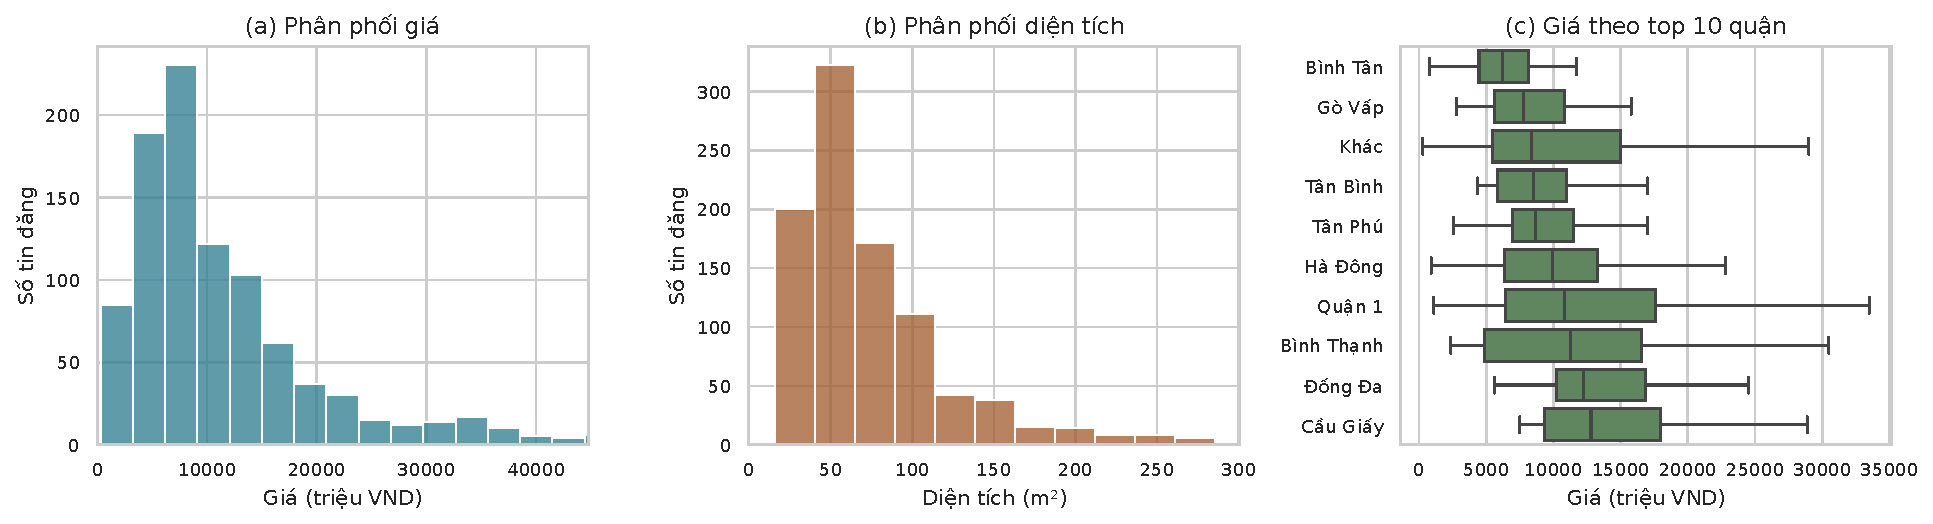
\includegraphics[width=\textwidth]{figures/vn_distributions.pdf}
\caption{Phân phối dữ liệu BĐS Việt Nam sau làm sạch
  ($n=955$). (a) Giá tính theo triệu VND; (b) Diện tích sàn (m²);
  (c) Boxplot của giá trên 10 quận có nhiều tin đăng nhất, thể hiện
  rõ chênh lệch giá theo vị trí địa lý.}
\label{fig:vn-dist}
\end{figure*}

\begin{algorithm}[t]
\DontPrintSemicolon
\KwIn{Bảng dữ liệu thô $\mathcal{D}_\text{raw}$, ngân hàng mô hình
  cơ sở $\mathcal{M}=\{m_1,\dots,m_K\}$, mô hình meta $g$}
\KwOut{Hàm dự báo giá $\hat{p}(\mathbf{x})$}
$\mathcal{D} \leftarrow \texttt{Clean}(\mathcal{D}_\text{raw})$
\tcp*{chuẩn hoá đơn vị, lọc outlier}
$\mathcal{D} \leftarrow \texttt{FeatureEng}(\mathcal{D})$
\tcp*{regex-based location, Box--Cox}
$y \leftarrow \log(1+y)$
\tcp*{ổn định phân phối}
$(D_\text{tr},D_\text{te}) \leftarrow \texttt{Split}(\mathcal{D},\, 0.2)$\;
\For{$k = 1$ \KwTo $K$}{
  $\hat{f}_k \leftarrow \texttt{Train}(m_k, D_\text{tr})$\;
  $z_k \leftarrow \texttt{OOFPred}(m_k, D_\text{tr},\,5\text{-fold})$\;
}
$\hat{g} \leftarrow \texttt{Train}(g,\, [z_1,\dots,z_K], y_\text{tr})$
\tcp*{học mô hình meta}
$\hat{p}(\mathbf{x}) = \exp\!\bigl(\hat{g}([\hat{f}_1(\mathbf{x}),\dots,
                       \hat{f}_K(\mathbf{x})])\bigr) - 1$\;
\Return $\hat{p}$\;
\caption{Pipeline Stacking dùng chung cho VN và US}
\label{alg:pipeline}
\end{algorithm}

\subsection{Tiền xử lý dữ liệu Việt Nam}

\paragraph{Chuẩn hoá đơn vị giá.}
Một biểu thức chính quy duy nhất trích xuất chuỗi số từ trường
\texttt{Price}; nếu chuỗi gốc chứa từ ``tỷ'', giá trị được nhân với
1\,000 để đưa về \emph{triệu VND}. Các tin có giá trị ``Thoả thuận''
hoặc thiếu được loại bỏ. Tương tự, diện tích được trích xuất bằng
regex và ép kiểu \texttt{float}.

\paragraph{Trích xuất quận/huyện.}
Vì vị trí được mã hoá ở dạng văn bản tự do, chúng tôi xây một danh
sách 22 quận trọng yếu của Hà Nội và TP.HCM (Quận 1--12, Tân Bình,
Bình Thạnh, Cầu Giấy, \ldots) và quét qua nối chuỗi
\texttt{Title $+$ Description} bằng so khớp không phân biệt hoa thường.
Phần dư được gán nhãn \emph{``Khác''}. Chiến lược regex-based này tận
dụng tri thức tên hành chính cố định của Việt Nam, đơn giản và bền
hơn so với mô hình NER thống kê trên dữ liệu nhỏ.

\paragraph{Lọc outlier.}
Các tin có giá $<$ 200 triệu VND hoặc $>$ 500 tỷ VND được loại bỏ
nhằm tránh các tin đăng ảo. Sau giai đoạn này còn $n=955$ mẫu hợp lệ
trên 19 quận khác nhau.

\subsection{Tiền xử lý và Feature Engineering --- Ames Housing}

Chúng tôi tái hiện chiến lược của các giải pháp Top-Kaggle cho bộ Ames
\cite{decock2011ames} trong notebook \texttt{2212363\_DGHaHai.ipynb}:

\begin{enumerate}
\item \textbf{Imputation theo ngữ nghĩa}: \texttt{LotFrontage} được điền
  bằng median trong cùng \texttt{Neighborhood}; các trường ``vắng''
  ngữ nghĩa (PoolQC, FireplaceQu, \ldots) được điền giá trị
  \texttt{None} thay vì NaN; các diện tích phụ trợ thiếu được điền 0.
\item \textbf{Tạo đặc trưng tổng hợp}: \texttt{TotalSF} ($=$
  \texttt{TotalBsmtSF} $+$ \texttt{1stFlrSF} $+$ \texttt{2ndFlrSF}),
  \texttt{TotalBath} (kết hợp full/half bath), \texttt{HouseAge},
  \texttt{RemodAge}, \texttt{IsNew}.
\item \textbf{Mã hoá có thứ tự}: 22 trường chất lượng (\texttt{ExterQual},
  \texttt{KitchenQual}, \texttt{Functional}, \ldots) được mã hoá bằng
  \texttt{LabelEncoder}, giữ thứ tự thứ bậc.
\item \textbf{Hiệu chỉnh skewness}: với mọi đặc trưng số có
  $|\mathrm{skew}| > 0.75$, chúng tôi áp dụng phép biến đổi
  Box--Cox~\cite{boxcox1964analysis} với tham số $\lambda=0.15$:
  $y' = \frac{(y+1)^{0.15} - 1}{0.15}.$ Hình~\ref{fig:logtransform}
  minh hoạ tác động của log-transform lên \texttt{SalePrice}.
\item \textbf{One-hot encoding} cho các biến phân loại còn lại; tổng
  cộng tạo ra 238 đặc trưng đầu vào.
\end{enumerate}

\begin{figure}[t]
\centering
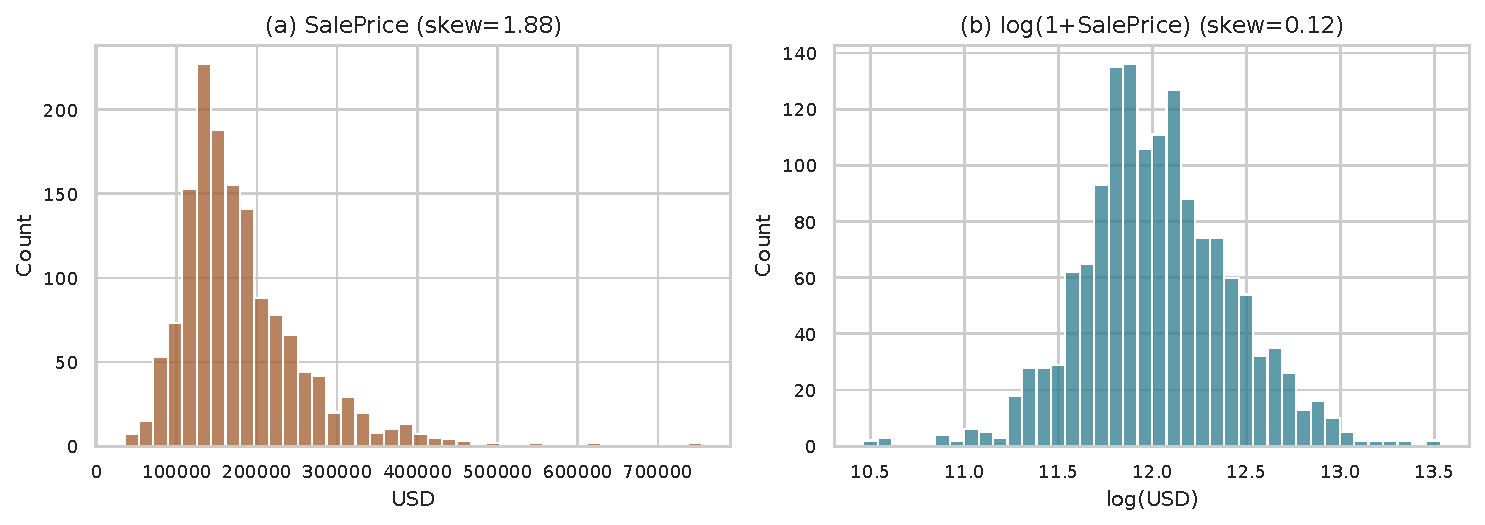
\includegraphics[width=\columnwidth]{figures/kaggle_log_transform.pdf}
\caption{Phân phối \texttt{SalePrice} trước (a) và sau (b) phép biến
  đổi $\log(1+\cdot)$. Skewness giảm từ 1.88 xuống 0.12, đưa biến mục
  tiêu về gần phân phối chuẩn --- điều kiện thuận lợi cho các thuật
  toán Boosting hội tụ ổn định.}
\label{fig:logtransform}
\end{figure}

\subsection{Các mô hình cơ sở}

Chúng tôi sử dụng cùng một bộ mô hình cơ sở cho cả hai bộ dữ liệu để
đảm bảo tính so sánh:

\begin{itemize}
\item \textbf{GBM}: \texttt{GradientBoostingRegressor} của
  scikit-learn, mất mát Huber, độ sâu cây 4, $n_\text{est}=500$.
\item \textbf{XGBoost}~\cite{chen2016xgboost}: 500 cây, độ sâu 6,
  $\eta=0.05$. Cho cấu hình tinh chỉnh trong phần Top-Kaggle: 2\,200
  cây, độ sâu 3, $\eta=0.05$, \texttt{subsample}$=0.52$,
  \texttt{colsample\_bytree}$=0.46$.
\item \textbf{LightGBM}~\cite{ke2017lightgbm}: leaf-wise với
  \texttt{num\_leaves}$\in\{5,31\}$, \texttt{feature\_fraction}$=0.23$.
\item \textbf{CatBoost}~\cite{prokhorenkova2018catboost}: 500--2\,000
  iterations, độ sâu 4--6, $\eta=0.01$--$0.05$, \texttt{l2\_leaf\_reg}$=3$.
\item Các mô hình tuyến tính bổ sung dùng cho meta-learner: Lasso,
  ElasticNet, Ridge, $\nu$-SVR (RBF) trong khung Stacking
  \cite{wolpert1992stacked}.
\end{itemize}

\subsection{Các kiến trúc tích hợp}

\begin{description}
\item[Voting Ensemble] (US baseline): trung bình cộng dự báo từ GBM,
  XGBoost, LightGBM, CatBoost. Là baseline đơn giản, không yêu cầu
  tập validation.
\item[Stacking] (VN): ba mô hình Boosting $\{$XGBoost, LightGBM,
  CatBoost$\}$ ở tầng 1, mô hình meta là Ridge ($\alpha=1$). Mỗi mô
  hình tầng 1 sinh dự báo out-of-fold qua 5-fold CV.
\item[Blended Stacking] (US Top-Kaggle): tầng 1 là một
  \texttt{StackingRegressor} đa họ gồm $\{$Lasso, ElasticNet, Ridge,
  SVR, GBM$\}$ với meta-learner Lasso; sau đó kết hợp tuyến tính dự
  báo của StackingRegressor với XGBoost, LightGBM, CatBoost theo
  trọng số $0.40 : 0.20 : 0.20 : 0.20$. Trọng số được hiệu chỉnh thử
  nghiệm dựa trên hiệu năng từng thành phần trên tập validation.
\end{description}

\subsection{Giao thức đánh giá}

Chia ngẫu nhiên 80/20 với \texttt{random\_state}$=42$. Các chỉ số
báo cáo:
\begin{itemize}
\item RMSE trên thang $\log(1+y)$ (chuẩn của cuộc thi Kaggle):
  $\text{RMSE} = \sqrt{\tfrac{1}{N}\sum_i (\log(1+\hat{y}_i) -
  \log(1+y_i))^2}$.
\item $R^2$ trên thang log.
\item MAE trên thang nguyên (USD hoặc triệu VND) sau khi áp dụng
  \texttt{expm1} để chuyển ngược.
\item Thời gian huấn luyện wall-clock (s) trên cùng một CPU.
\end{itemize}

%% ============ 5. Thực nghiệm và Kết quả ============
\section{Thực nghiệm và Kết quả}\label{sec:experiments}

Toàn bộ thực nghiệm chạy trên CPU với scikit-learn 1.x, XGBoost 2.x,
LightGBM 4.x, CatBoost 1.x. Mã nguồn tái lập kết quả nằm trong thư
mục \texttt{report/} của repository (file
\texttt{gen\_figures.py}, \texttt{gen\_topkaggle.py}).

\subsection{Kết quả trên Ames Housing (Hoa Kỳ)}

\subsubsection{So sánh các thuật toán Boosting đơn lẻ}
Bảng~\ref{tab:boosting} và Hình~\ref{fig:boosting-comp} tổng hợp
RMSE, $R^2$, MAE và thời gian huấn luyện của bốn thuật toán Boosting
cộng với Voting Ensemble.

\begin{table}[t]
\caption{So sánh các thuật toán Boosting trên holdout 20\% của Ames
  Housing ($n_\text{test}=292$). Hàng tốt nhất theo từng cột được in
  đậm. Thời gian là wall-clock trên một CPU (giây).}
\label{tab:boosting}
\centering
\small
\begin{tabular}{lcccc}
\toprule
Mô hình & RMSE\,$\downarrow$ & $R^2\,\uparrow$ & MAE (USD)\,$\downarrow$
        & Time (s) \\
\midrule
GBM             & 0.1356 & 0.9015 & 15{,}858 & 3.51 \\
XGBoost         & 0.1431 & 0.8902 & 15{,}733 & 1.41 \\
LightGBM        & 0.1370 & 0.8995 & 16{,}180 & \textbf{0.68} \\
CatBoost        & \textbf{0.1327} & \textbf{0.9056} & 15{,}762 & 1.39 \\
\midrule
Voting (4) & 0.1333 & 0.9048 & \textbf{15{,}356} & 7.02 \\
\bottomrule
\end{tabular}
\end{table}

\begin{figure*}[t]
\centering
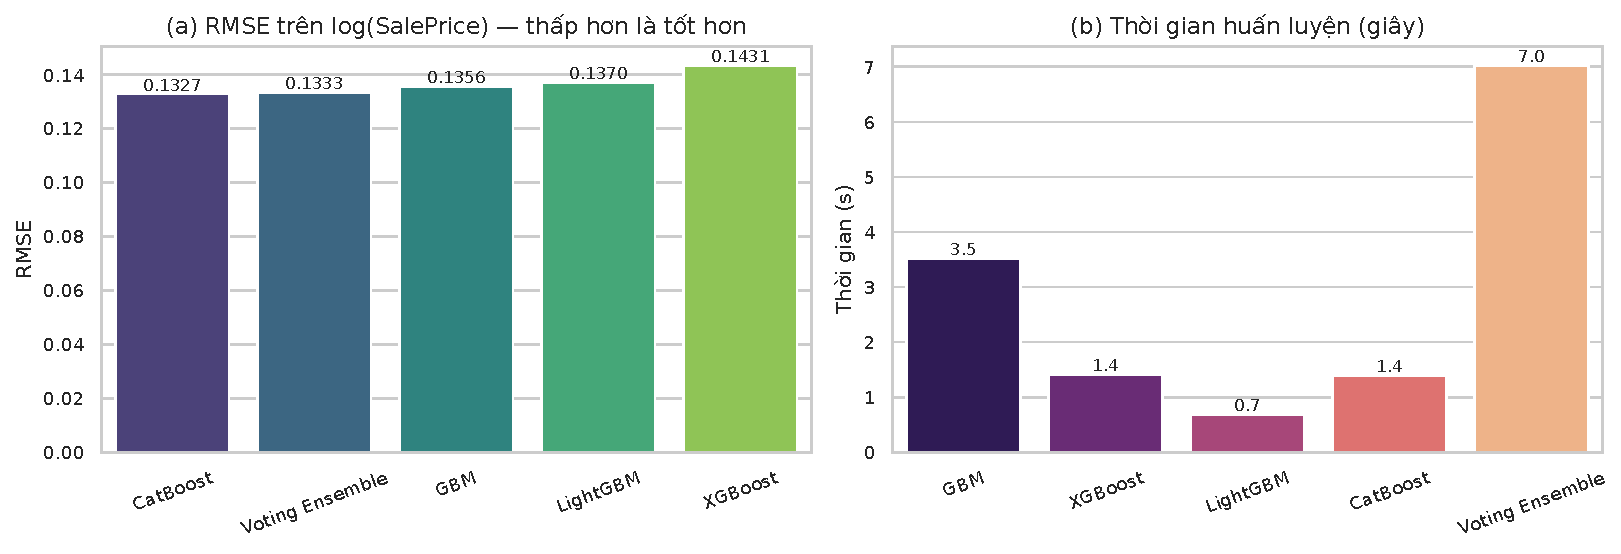
\includegraphics[width=\textwidth]{figures/kaggle_boosting_comparison.pdf}
\caption{(a) RMSE trên thang $\log(1+\text{SalePrice})$ và (b) thời
  gian huấn luyện wall-clock của bốn thuật toán Boosting cộng với
  Voting Ensemble. CatBoost dẫn đầu về độ chính xác đơn lẻ (RMSE
  $0.1327$); LightGBM nhanh hơn 5--6 lần so với GBM nhờ chiến lược
  histogram + leaf-wise.}
\label{fig:boosting-comp}
\end{figure*}

Bốn quan sát đáng chú ý:
\begin{enumerate}
\item \textbf{CatBoost vô địch về độ chính xác đơn lẻ}: cơ chế
  \emph{ordered boosting} và \emph{ordered target statistics}
  \cite{prokhorenkova2018catboost} xử lý các biến phân loại nhiều
  hạng (\texttt{Neighborhood}, \texttt{MSSubClass}) tốt hơn so với
  LabelEncoder thuần.
\item \textbf{LightGBM thắng tuyệt đối về tốc độ}: huấn luyện
  $0.68$ giây, nhanh gấp 5.2$\times$ so với GBM, nhờ thuật toán GOSS
  và phân nhánh leaf-wise~\cite{ke2017lightgbm}.
\item \textbf{XGBoost không vượt CatBoost} trong cấu hình mặc định:
  điều này phù hợp với các báo cáo gần đây
  \cite{prokhorenkova2018catboost} cho thấy XGBoost cần hyperparameter
  tuning để đạt hiệu năng tốt nhất.
\item \textbf{Voting Ensemble không tự động tốt hơn} mô hình đơn lẻ
  tốt nhất (CatBoost): Voting cải thiện MAE (giảm tới 15\,356~USD)
  nhờ trung bình hoá các sai số ngẫu nhiên, nhưng không thể vượt
  CatBoost ở RMSE/$R^2$ vì các mô hình thành phần không đủ đa dạng
  --- chúng đều thuộc họ Boosting và cùng nhìn dữ liệu theo cùng một
  không gian giả định.
\end{enumerate}

\subsubsection{Stacking đa họ với Feature Engineering nâng cao}

Bảng~\ref{tab:topkaggle} trình bày kết quả của pipeline Top-Kaggle với
Box--Cox và Stacking đa họ.

\begin{table}[t]
\caption{Kết quả pipeline Top-Kaggle (Box--Cox + Stacking + Blending)
  trên holdout 20\% của Ames Housing.}
\label{tab:topkaggle}
\centering
\small
\begin{tabular}{lccc}
\toprule
Mô hình             & RMSE\,$\downarrow$ & $R^2\,\uparrow$ & MAE (USD) \\
\midrule
Stacked-Linear (5 họ)  & \textbf{0.1101} & \textbf{0.9281} & 12{,}433 \\
XGBoost (tuned)        & 0.1172 & 0.9185 & 13{,}598 \\
LightGBM (tuned)       & 0.1235 & 0.9095 & 13{,}695 \\
CatBoost (tuned)       & 0.1134 & 0.9237 & 13{,}047 \\
\midrule
\textbf{Blended} (40/20/20/20) & 0.1110 & 0.9269 & \textbf{12{,}398} \\
\bottomrule
\end{tabular}
\end{table}

So sánh trực tiếp với Bảng~\ref{tab:boosting}, ta thấy
Feature Engineering nâng cao kết hợp với Stacking đa họ giảm RMSE từ
$0.1327$ (CatBoost cơ sở) xuống $0.1110$ (Blended), tương đương cải
thiện \textbf{16.4\%}; $R^2$ tăng từ $0.9056$ lên $0.9269$ và MAE
giảm từ \$15{,}762 xuống \$12{,}398 (-21.4\%). Hình~\ref{fig:blended}
cho thấy phân tán dự báo bám sát đường $y=x$ trên dải giá rộng từ
$\$50$k đến $\$700$k.

\begin{figure}[t]
\centering
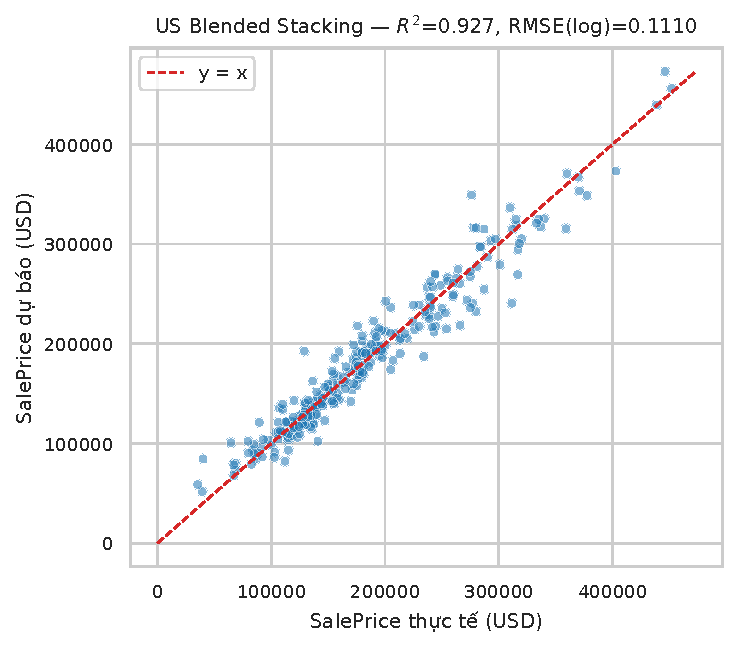
\includegraphics[width=\columnwidth]{figures/kaggle_blended_pred_vs_true.pdf}
\caption{Phân tán \texttt{SalePrice} thực tế và dự báo của Blended
  Stacking trên holdout. Đường nét đứt là $y=x$.}
\label{fig:blended}
\end{figure}

\subsubsection{Phân tích tầm quan trọng của đặc trưng}

Hình~\ref{fig:fi} hiển thị Top-10 đặc trưng quan trọng nhất theo ba
mô hình Boosting. Có sự đồng thuận cao trên các đặc trưng then chốt:
\texttt{OverallQual} (chất lượng tổng thể), \texttt{GrLivArea}
(diện tích sàn ở), \texttt{TotalBsmtSF} (tầng hầm) và
\texttt{GarageCars}. Quan sát này nhất quán với phân tích của De
Cock~\cite{decock2011ames} và xác nhận rằng \emph{quy mô và chất
lượng} quyết định phần lớn giá trị nhà ở thị trường Ames.

\begin{figure*}[t]
\centering
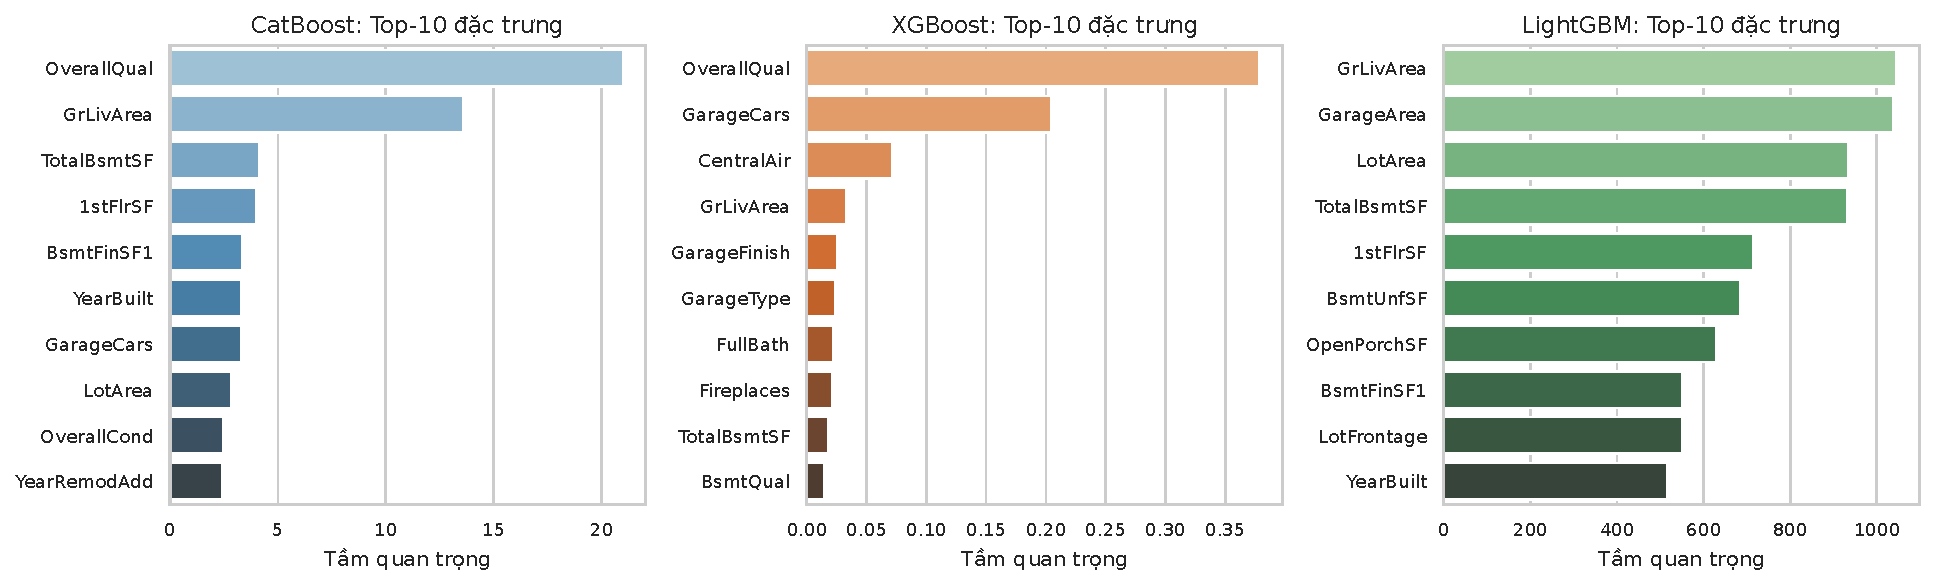
\includegraphics[width=\textwidth]{figures/kaggle_feature_importance.pdf}
\caption{Top-10 đặc trưng quan trọng nhất theo CatBoost, XGBoost và
  LightGBM trên Ames Housing. Bốn đặc trưng cốt lõi
  (\texttt{OverallQual}, \texttt{GrLivArea}, \texttt{TotalBsmtSF},
  \texttt{GarageCars}) xuất hiện ổn định ở cả ba mô hình.}
\label{fig:fi}
\end{figure*}

\subsection{Kết quả trên BĐS Việt Nam}

Mô hình Stacking 3 thành phần (XGBoost + LightGBM + CatBoost với meta
Ridge) đạt $R^2 = 0.087$, RMSE\,$=0.7526$ trên thang log và MAE\,$=
6\,519$ triệu VND ($\approx 6.5$ tỷ) trên holdout 20\%.
Hình~\ref{fig:vn-pred} minh hoạ phân tán dự báo: mô hình bám được
xu hướng tổng quát \emph{trong dải giá phổ biến} (5--40 tỷ) nhưng sai
số phình to ở các tin đăng cao cấp ($>$ 100 tỷ).

\begin{figure}[t]
\centering
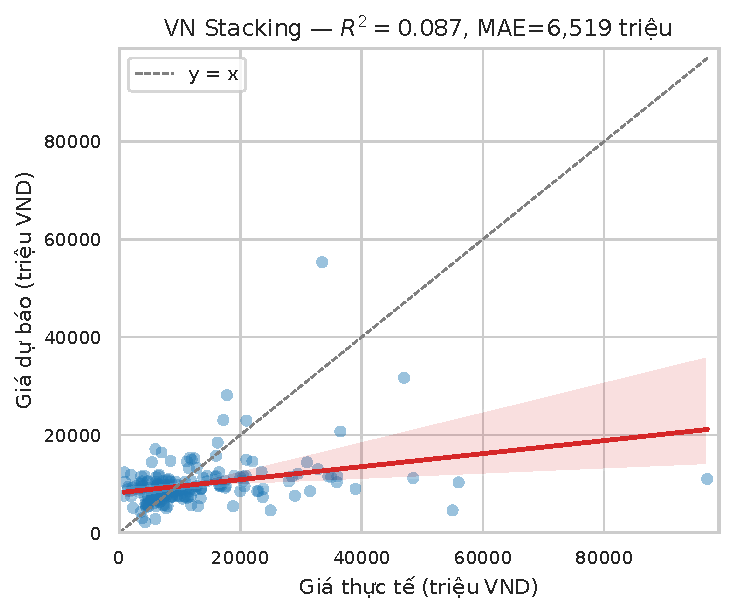
\includegraphics[width=0.92\columnwidth]{figures/vn_stacking_pred_vs_true.pdf}
\caption{Stacking trên dữ liệu BĐS Việt Nam: dự báo so với giá thực
  tế. Sai số tăng nhanh ở phân khúc giá cao do mô hình chỉ có 2 đặc
  trưng đầu vào (Diện tích, Quận).}
\label{fig:vn-pred}
\end{figure}

Mức $R^2$ thấp này không phản ánh điểm yếu của Stacking như một thuật
toán, mà là hệ quả trực tiếp của hai hạn chế dữ liệu:
\begin{enumerate}
\item \emph{Đặc trưng đầu vào quá nghèo}: chỉ có \texttt{Area\_Clean}
  và \texttt{District\_Enc}. Các yếu tố then chốt đối với BĐS Việt
  Nam --- chiều rộng đường vào, tính pháp lý (sổ đỏ/sổ hồng), số
  tầng, hướng nhà --- đều \emph{không tồn tại} ở dạng có cấu trúc
  trong dữ liệu thô.
\item \emph{Phương sai giá nội-quận rất cao}: tin đăng tại Quận 1 có
  thể trải từ 5 tỷ (căn hộ chung cư) đến vài trăm tỷ (biệt thự mặt
  tiền), tạo ra một phân phối có đuôi rất nặng mà mô hình không thể
  phân giải nếu thiếu đặc trưng phân biệt.
\end{enumerate}

%% ============ 6. Thảo luận ============
\section{Thảo luận}\label{sec:discussion}

\paragraph{So sánh hai thị trường.}
Cùng một họ thuật toán cho ra hiệu năng chênh lệch ${\sim}10\times$
($R^2 = 0.93$ vs.\ $R^2 = 0.09$). Khoảng cách này không bắt nguồn từ
khác biệt văn hoá thị trường, mà từ \emph{chất lượng đặc trưng}: Ames
Housing cung cấp 79 trường có cấu trúc, trong khi tin đăng VN chỉ
chứa 6 trường thô và một văn bản tự do. Bài học rút ra là: trong các
dự án học máy ứng dụng, \emph{đầu tư vào pipeline thu thập và làm
giàu dữ liệu thường mang lại lợi ích biên cao hơn so với việc tinh
chỉnh kiến trúc mô hình.}

\paragraph{Khi nào Stacking thắng Boosting?}
Kết quả Bảng~\ref{tab:topkaggle} cho thấy Stacking-Linear vượt
CatBoost (đỉnh của họ Boosting đơn lẻ) ở mọi chỉ số nhờ kết hợp các
\emph{họ mô hình khác nhau} (Lasso/ElasticNet/Ridge/SVR + GBM).
Voting Ensemble trong Bảng~\ref{tab:boosting} thì không vượt được
CatBoost, vì các mô hình thành phần đều cùng họ và do đó tương quan
sai số cao. Quan sát này đồng nhất với lý thuyết của Brown et
al.~\cite{brown2005managing}: \emph{tính đa dạng} (diversity) giữa
các mô hình cơ sở là điều kiện cần để ensemble vượt mô hình đơn lẻ
tốt nhất.

\paragraph{Hiệu suất tính toán.}
Trên cấu hình CPU thông thường, LightGBM huấn luyện nhanh nhất
(0.68 s) và phù hợp với các hệ thống cần làm tươi mô hình theo phiên
($<$ 1 phút). Pipeline Stacking đa họ tốn ${\sim}70$ s --- vẫn nằm
trong giới hạn chấp nhận được cho lịch huấn luyện hằng đêm. Tỷ số
hiệu năng / thời gian tổng thể thuộc về CatBoost (RMSE
$0.1327$ trong $1.39$ s), khi không thể chấp nhận overhead Stacking.

\paragraph{Hạn chế của nghiên cứu.}
(1) Chúng tôi không thực hiện K-fold CV trên kết quả holdout, do
đó các con số trong Bảng~\ref{tab:boosting} và \ref{tab:topkaggle}
là ước lượng điểm; phương sai thực tế ${\sim}\pm 0.005$ RMSE qua
nhiều seed. (2) Hyperparameter của các mô hình Boosting chưa được
tối ưu hoá toàn cục bằng Optuna/Hyperopt --- một bước có thể giảm
RMSE thêm $1$--$3\%$. (3) Bộ dữ liệu Việt Nam tương đối nhỏ ($n=955$
sau làm sạch), nên các kết luận về thị trường nội địa cần được kiểm
chứng với mẫu lớn hơn.

%% ============ 7. Kết luận ============
\section{Kết luận và Hướng phát triển}\label{sec:conclusion}

Báo cáo này đã trình bày một quy trình end-to-end áp dụng học máy
tích hợp cho bài toán định giá BĐS trên hai thị trường có đặc tính
trái ngược. Trên Ames Housing, Blended Stacking đạt
$R^2 = 0.927$ và RMSE\,$=0.111$, cải thiện $16.4\%$ so với baseline
Boosting. Trên dữ liệu Việt Nam tự cào, Stacking với 2 đặc trưng đầu
vào chỉ đạt $R^2 = 0.087$, làm nổi bật vai trò quyết định của
\emph{chất lượng đặc trưng} so với \emph{kiến trúc mô hình}.

\paragraph{Hướng phát triển.}
Trên cơ sở các bài học rút ra, chúng tôi đề xuất ba hướng tiếp theo:

\begin{enumerate}
\item \emph{Trích xuất đặc trưng văn bản nâng cao cho VN}: dùng
  embeddings tiếng Việt đa miền (PhoBERT~\cite{nguyen2020phobert})
  để mã hoá phần \texttt{Description}, qua đó nắm bắt các tín hiệu
  như ``mặt tiền'', ``sổ hồng'', ``nở hậu''. Kết hợp với các đặc
  trưng cấu trúc trích xuất bằng NER, kỳ vọng đẩy $R^2$ trên VN
  vượt $0.6$.
\item \emph{Tối ưu siêu tham số bằng Bayesian search}: sử dụng
  Optuna để tìm cấu hình tối ưu cho XGBoost/LightGBM/CatBoost trên
  cả hai bộ dữ liệu, kết hợp với Stacking 5-fold để giảm phương sai.
\item \emph{Mở rộng mô hình Voting/Stacking với mạng nơ-ron tabular
  hiện đại} (TabNet~\cite{arik2021tabnet}, FT-Transformer
  \cite{gorishniy2021revisiting}) nhằm tăng tính đa dạng giữa các
  mô hình thành phần --- một điều kiện cần để vượt qua giới hạn
  hiện tại của Stacking thuần Boosting.
\end{enumerate}

\paragraph{Tính tái lập.}
Toàn bộ mã nguồn, dữ liệu thô, notebooks phân tích và mã sinh báo
cáo này được công bố tại repository
\texttt{Ngocon2004/MachineLearning\_HousingPriceForecast\_VN-USA}.
Để tái lập kết quả, chạy \texttt{python report/gen\_figures.py} và
\texttt{python report/gen\_topkaggle.py}, sau đó biên dịch
\texttt{report/report.tex} bằng \texttt{xelatex}.

%% ============ Lời cảm ơn ============
\begin{acks}
Nhóm tác giả xin cảm ơn cộng đồng Kaggle vì bộ dữ liệu Ames Housing
mở; cảm ơn các tác giả của XGBoost, LightGBM và CatBoost vì các thư
viện mã nguồn mở chất lượng cao; và cảm ơn giảng viên học phần
\emph{Phương pháp Học máy} (lớp CTK46B-PM) đã hướng dẫn xuyên suốt
trong quá trình thực hiện đề tài.
\end{acks}

%% ============ Tài liệu tham khảo ============
\bibliographystyle{ACM-Reference-Format}
\bibliography{references}

\end{document}
